\documentclass[main]{subfiles}

\begin{document}
\subsection{Modul To}
Efter at have målt  switchen, som beskrevet i \cref{dataopsamling2}, konkluderes det, at system er hurtig nok til at måle et signal. Herefter måles laserstrålens waist, ved at logge  den transmitterede intensitet som funktion af mikrometerskrue. Dette ses på \cref{fig:graf3}.
\begin{figure}[H]
    \centering
    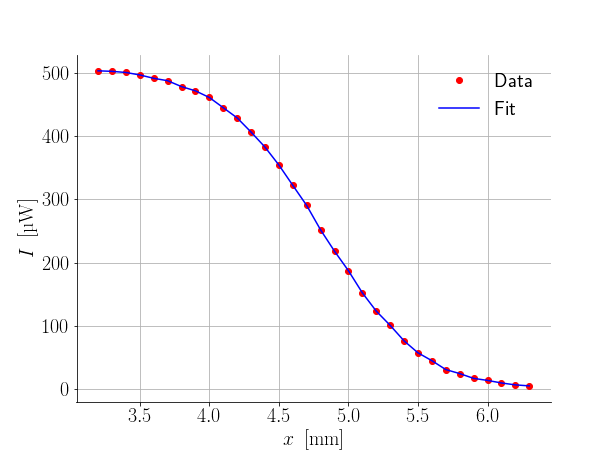
\includegraphics[width=\linewidth]{tegninger/graf3.png}
    \caption{}
    \label{fig:graf3}
\end{figure}

\end{document}
